\documentclass[conference]{IEEEtran}
% \IEEEoverridecommandlockouts
% The preceding line is only needed to identify funding in the first footnote. If that is unneeded, please comment it out.
\usepackage{cite}
\usepackage{amsmath,amssymb,amsfonts}
\usepackage{algorithmic}
\usepackage{graphicx}
\usepackage{textcomp}
\usepackage{xcolor}
\usepackage{siunitx}
\def\BibTeX{{\rm B\kern-.05em{\sc i\kern-.025em b}\kern-.08em
T\kern-.1667em\lower.7ex\hbox{E}\kern-.125emX}}
\begin{document}

\title{Energy-Efficient Communication in UAV-assisted Batteryless WSNs Using Passive Wake-up Radios}

\author{
  \IEEEauthorblockN{Miguel Brandt, Adriano Branco, and Markus Endler}
  \IEEEauthorblockA{\textit{Department of Informatics} \\
    \textit{Pontifical Catholic University of Rio de Janeiro} \\
    Rio de Janeiro, Brazil \\
    miguelperes@aluno.puc-rio.br,\\
  \{abranco,endler\}@inf.puc-rio.br}
  \and
  \IEEEauthorblockN{Kelvin Bittencourt}
  \IEEEauthorblockA{\textit{Department of Electrical Engineering} \\
    \textit{Pontifical Catholic University of Rio de Janeiro} \\
    Rio de Janeiro, Brazil \\
  kelvinbitt@aluno.puc-rio.br}
}

\maketitle

\begin{abstract}
  A number of studies have been proposed to tackle the task of monitoring large areas by deploying a wireless sensor network. When communication infrastructure is unavailable, or the region is not easily accessible, data can be retrieved from such networks by using Unmanned Aerial Vehicles (UAVs) as gateways to a base station, thus creating a UAV-assisted Wireless Sensor Network (UAV-WSN). However, providing regular maintenance for an extensive, scattered WSN is impractical, leading to devices with limited service life, usually tied to their battery lifespan. Consequently, they are often treated as disposable, and as a result, become chemical waste. In this ongoing study, we explore the integration of batteryless sensors powered by energy harvesting (EH) within UAV-WSNs. Since energy-efficient sensors cannot be continuously powered on, we begin by investigating techniques for establishing communication between sensors in a sleep state and UAVs, and ultimately focus on passive wake-up radios, proposing a simple design and discussing the results of real-world experiments.
\end{abstract}

\section{Introduction}

Mobile data sink nodes have been increasingly used to support wireless sensor networks in remote or hard-to-reach areas\cite{gradys,uav_wsn_survey,survey_monitoring_uavwsn}. In UAV-WSNs, UAVs act as dynamic gateways, enabling data transfer from localized sensors to a base station and relaying data to the cloud for further processing. This approach can be valuable for applications such as environmental monitoring\cite{flood_forecasting_uavwsn,rural_environmental_monitoring_uavwsn}, precision agriculture\cite{agriculture_uavwsn}, and infrastructure inspection\cite{structure_monitoring_uavwsn}.

One of the challenges with WSNs in remote areas is the reliance on battery-powered sensors, which have limited lifespans and contribute to environmental waste (CITE). Energy harvesting offers a potential solution by enabling sensors to operate without batteries, instead drawing energy from ambient sources like solar or radiofrequency (RF) waves (CITE). However, EH systems pose their own difficulties, including limited and fluctuating power availability, dependence on environmental conditions, and the need for efficient energy management(CITE). These limitations often lead to intermittent operation, where sensors cannot be continuously active(CITE), making it necessary to employ communication strategies that minimize energy consumption.

\section{Energy-Efficient Communication}

Traditional duty cycling reduces energy consumption in wireless sensor networks (WSNs) by periodically switching sensors between active and sleep states(CITE). However, this method introduces several drawbacks, including overhearing, increased latency, packet loss, synchronization complexity, and energy inefficiency during low activity periods(CITE). Wake-up receiver (WuRx)-based solutions offer a more efficient alternative by allowing sensors to remain in deep sleep until activated by an external signal, significantly reducing energy consumption(CITE). Additionally, WuRxs can be configured for addressed wake-up, ensuring that only specific sensors are activated by the wake-up signal, thereby reducing unnecessary energy expenditure.(CITE)

Various WuRx approaches exist, including radiofrequency, optical, and acoustic receivers, each suited for specific applications\cite{overview_wurx_survey}. Optical receivers are suitable for indoor scenarios where RF is undesirable\cite{optical_wurx}, notably in hospital operating rooms or production lines, while acoustic receivers are proposed for monitoring the health of critical infrastructure, for example, bridges, by scanning the structure's acoustic signature\cite{acoustic_wurx_structure}, as well as for communication with underwater devices where RF signals cannot penetrate effectively\cite{acoustic_wurx_underwater}. Nevertheless, in the context of UAV-WSNs, wake-up radios (WuRs) are particularly advantageous due to their ability to provide reliable, energy-efficient, long-range activation without the need for line-of-sight(CITE).

Considering the constraints of an EH-powered sensor network, we focused on passive WuR designs that operate without relying on any dedicated power source, enabling reliable operation even under scarce energy conditions. Figure \ref{fig:drone_over_sensor} illustrates an outdoor test scenario where a UAV with an amplified transmitter approaches a solar EH-powered sensor node that utilizes our passive WuR prototype, detailed in the subsequent section.

\begin{figure}[htbp]
  \centerline{\includegraphics[width=0.8\linewidth]{drone_flying_over_sensor.jpg}}
  \caption{Autonomous UAV approaching a batteryless sensor}
  \label{fig:drone_over_sensor}
\end{figure}

\section{Experiment and Results}

\subsection{Experimental Setup}

In order to conduct experiments, we assembled a passive wake-up radio on a protoboard using off-the-shelf components, based on a voltage doubler circuit, with a 17.3~cm quarter-wave monopole copper wire antenna, as we expect to receive a 433~MHz signal. For experiments with commercial antennas, a 50~$\Omega$ matching network is included.

Since the primary function of the WuR is to trigger an interrupt in the sensor's GPIO ports, we've also added a 1N4728A voltage clamping Zener diode of 3.3~V to prevent accidental overvoltage on the microcontroller. The circuit is depicted in Figure \ref{fig:receiver}.

\begin{figure}[htbp]
  \centerline{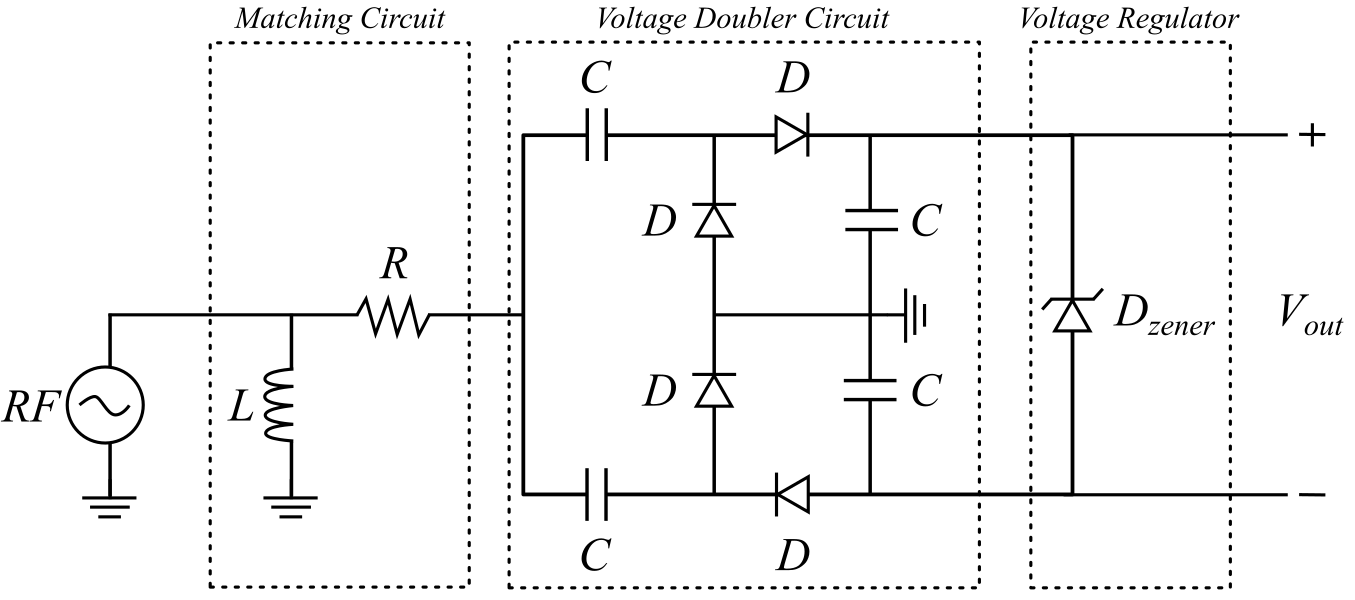
\includegraphics[width=1\linewidth]{receiver.png}}
  \caption{Passive wake-up radio prototype schematic}
  \label{fig:receiver}
\end{figure}

In this instance, we performed in-lab measurements with the transmitter powered directly by a DC power supply. The transmitter is a Texas Instruments (TI) CC1101 radio connected to an Espressif ESP32 microcontroller, which is programmed to continuously send a carrier wave with arbitrary data at its maximum power of +12~dBm, in the 433~MHz frequency range. The receiver is connected to an oscilloscope for measuring output voltage, as we hope to achieve at least 2.3~V, the minimum threshold for interrupt detection by most low-power microcontrollers, namely our TI MSP430-equipped sensor node.

Although initial tests were performed indoors, we've also built an autonomous, programmable, and modular UAV, as seen in Figure \ref{fig:drone_over_sensor}, to assess more realistic scenarios.

\subsection{Preliminary Findings}

Experiments revealed that the transmitter's output power was unable to charge the receiver's capacitors at a significant rate, except when their antennas were less than 1~cm apart, at which point we attribute the energy transfer to near-field coupling, rather than far-field RF harvesting. Because the UAV cannot hover on top of the receiver for too long, it is essential that the voltage rapidly reaches 2.3~V. Ideally, the UAV would fly over the sensor and collect the necessary data without decelerating.

As a point of reference, we've also performed tests with a commercial 433~MHz handheld transceiver capable of 2-3~W (33-34.7~dBm) output power, which was able to quickly generate an interrupt on the receiver at a 30~cm distance while transmitting. Based on these observations, we believe that incorporating an active amplifier of similar power into our original setup is necessary, either in the transmitter, using the UAV's battery as a power source, or at the receiver's $V_{\text{out}}$, borrowing power from the sensor's energy harvester. We plan to compare both solutions in our next phase of research.

\section{Conclusion}

The initial findings of this study highlight the challenges of using passive wake-up radios effectively. While the in-lab experiments confirmed their feasibility, achieving efficient energy transfer at practical distances remains a complex issue. Additional development in the energy transmission and harvesting process is necessary to achieve improved outcomes, with subsequent studies focusing on more effective antenna designs and circuit optimization for RF operation, as well as evaluating the introduction of addressing capabilities to prevent unwanted wake-ups.

Moreover, future efforts should present results from extensive outdoor tests using autonomous UAVs to evaluate the impact of external variables, such as electromagnetic interference from the UAV's motors and the communication reliability with a non-stationary transmitter.

By addressing these challenges, we hope to advance the practical implementation of sustainable, batteryless sensor networks within a UAV-WSN setting.

\bibliographystyle{IEEEtran}
\bibliography{references}

\end{document}
